% Please add the following required packages to your document preamble:
% \usepackage[table,xcdraw]{xcolor}
% If you use beamer only pass "xcolor=table" option, i.e. \documentclass[xcolor=table]{beamer}
\begin{table}[H]
\centering
\caption{Índices de Sobol e coeficientes de erro correspondentes para análise de
  sensitividade com 70.000 parametrizações.}
\label{apptab1}
\begin{tabular}{
>{\columncolor[HTML]{EFEFEF}}l |r|r|r|r|}
\cline{2-5}
\cellcolor[HTML]{FFFFFF}                                 & \cellcolor[HTML]{C0C0C0}S1 & \cellcolor[HTML]{C0C0C0}S1\_conf & \cellcolor[HTML]{C0C0C0}ST & \cellcolor[HTML]{C0C0C0}ST\_conf \\ \hline
\multicolumn{1}{|l|}{\cellcolor[HTML]{EFEFEF}N}          & -0.000960                  & 0.003781                         & 0.009199                   & 0.001663                         \\ \hline
\multicolumn{1}{|l|}{\cellcolor[HTML]{EFEFEF}n\_issues}  & 0.386739                   & 0.031786                         & 0.430023                   & 0.021672                         \\ \hline
\multicolumn{1}{|l|}{\cellcolor[HTML]{EFEFEF}p}          & 0.058764                   & 0.010221                         & 0.084306                   & 0.005647                         \\ \hline
\multicolumn{1}{|l|}{\cellcolor[HTML]{EFEFEF}\(\sigma\)} & 0.392436                   & 0.030570                         & 0.462914                   & 0.029143                         \\ \hline
\multicolumn{1}{|l|}{\cellcolor[HTML]{EFEFEF}\(\rho\)}   & 0.065982                   & 0.014993                         & 0.121552                   & 0.007549                         \\ \hline
\multicolumn{1}{|l|}{\cellcolor[HTML]{EFEFEF}p\_intran}  & 0.002966                   & 0.004155                         & 0.010803                   & 0.001572                         \\ \hline
\end{tabular}
\fonte{ O autor.}
\end{table}


\begin{figure}[H]
    \centering
    \begin{subfigure}[b]{0.49\textwidth}
        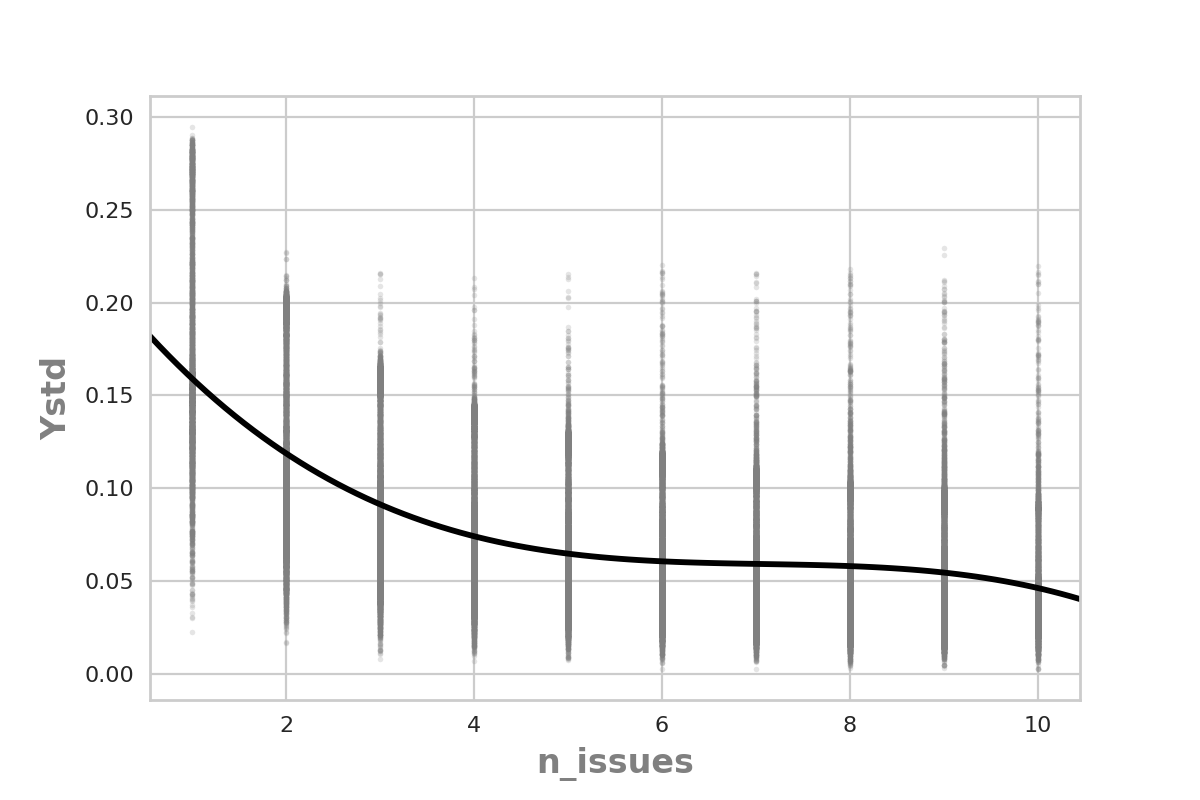
\includegraphics[width=\textwidth]{ims/nlregressions/nlregressionmutatingon_issues.png}
    \end{subfigure}
    \begin{subfigure}[b]{0.49\textwidth}
        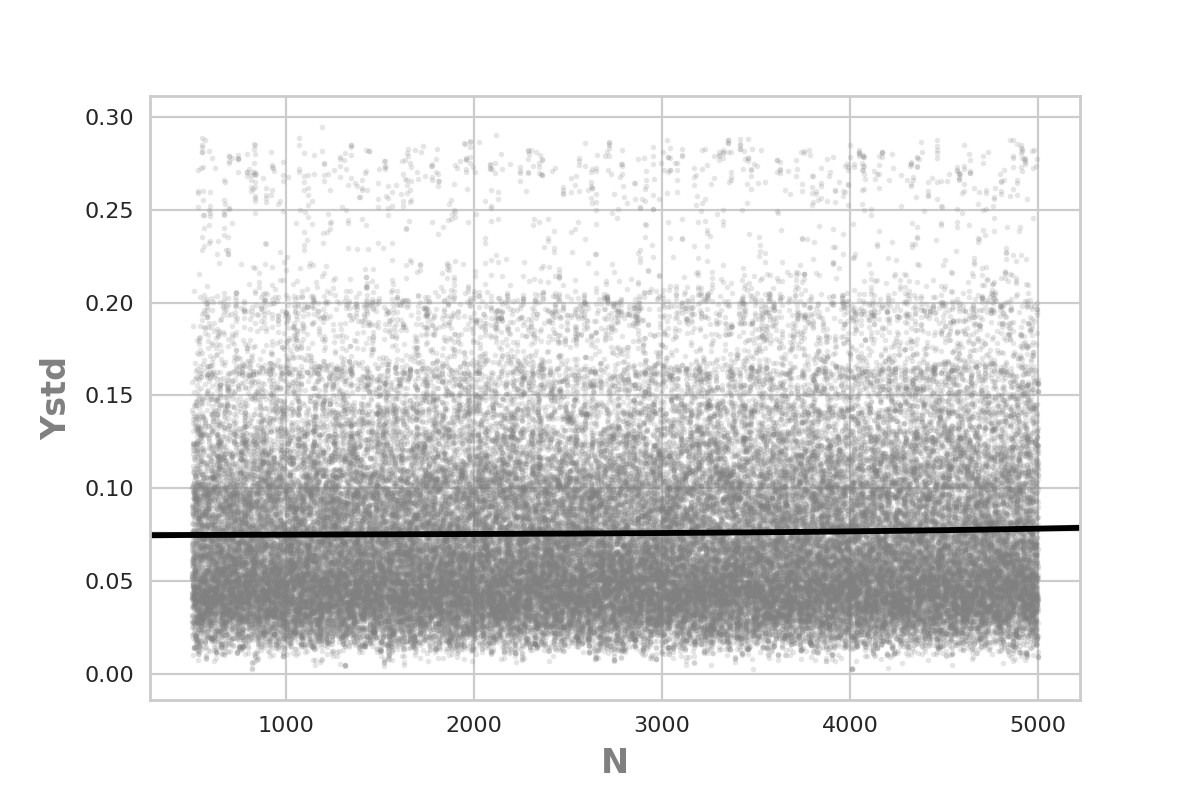
\includegraphics[width=\textwidth]{ims/nlregressions/nlregressionmutatingoN.png}
    \end{subfigure}

    \begin{subfigure}[b]{0.49\textwidth}
        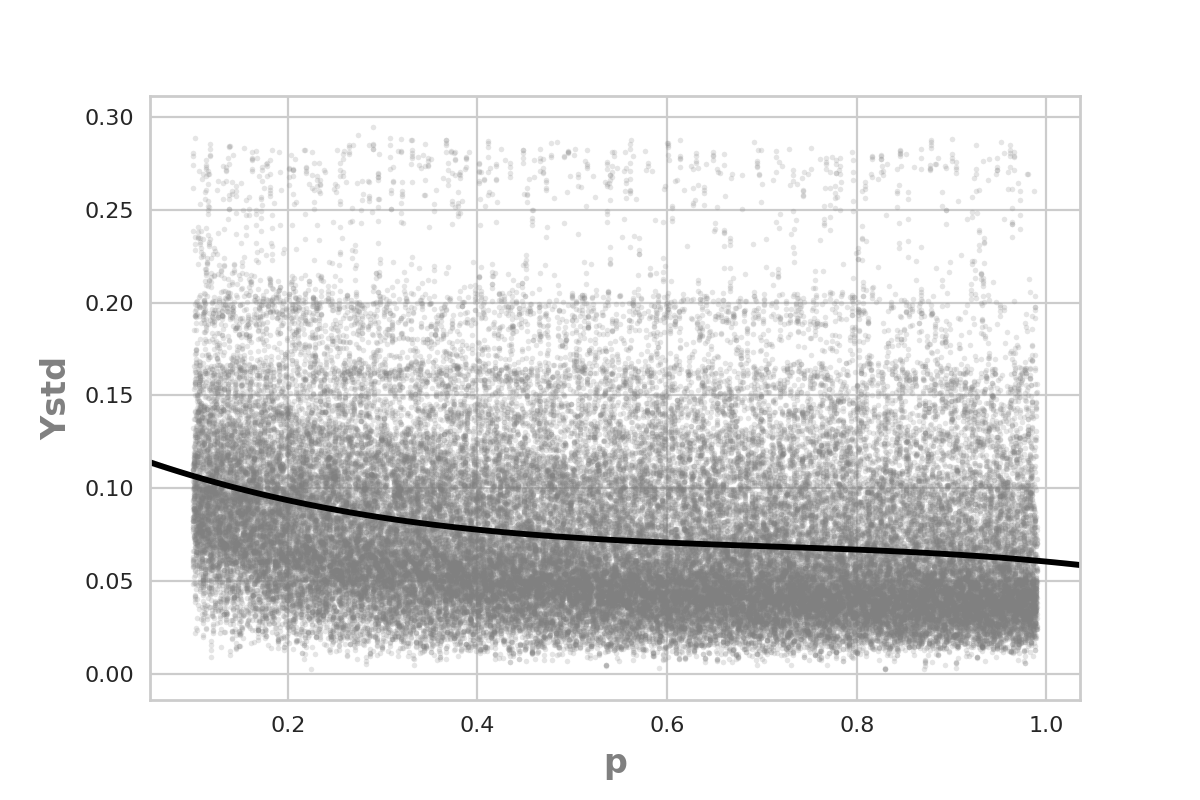
\includegraphics[width=\textwidth]{ims/nlregressions/nlregressionmutatingop.png}
      \end{subfigure}
          \begin{subfigure}[b]{0.49\textwidth}
            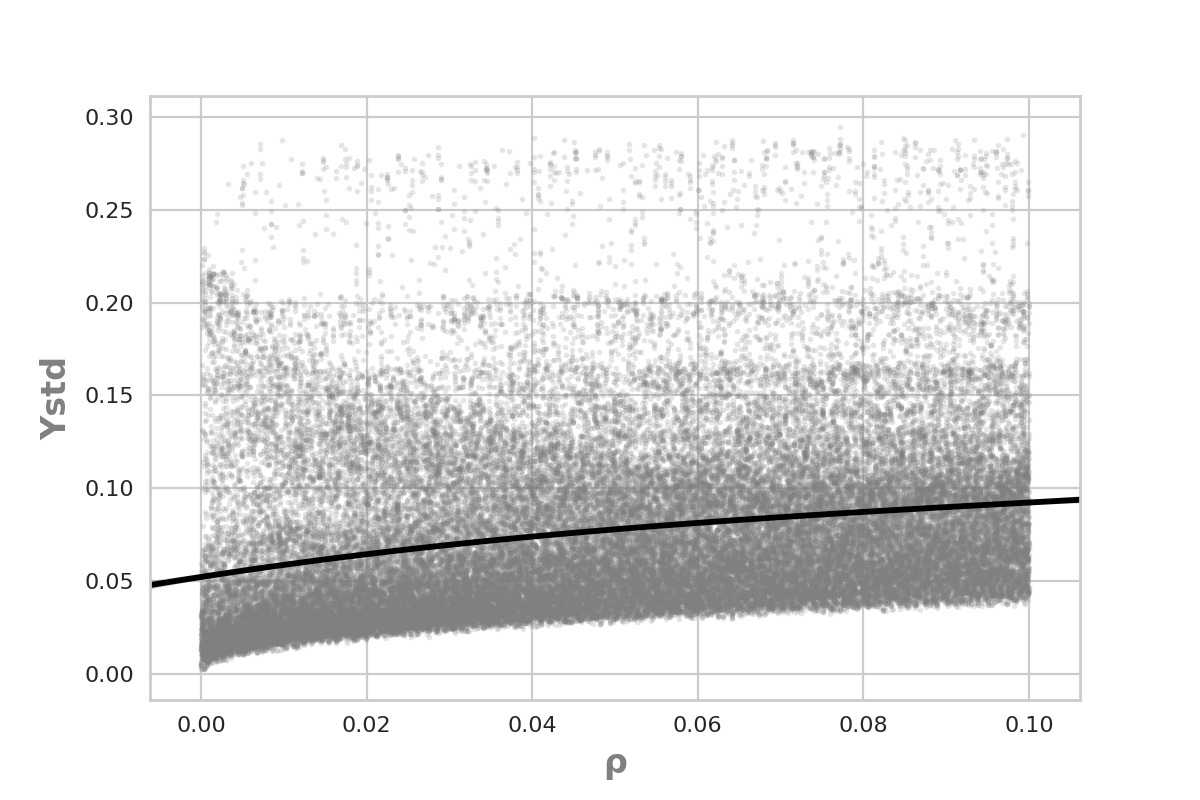
\includegraphics[width=\textwidth]{ims/nlregressions/nlregressionmutatingorho.png}
      \end{subfigure}

                \begin{subfigure}[b]{0.49\textwidth}
            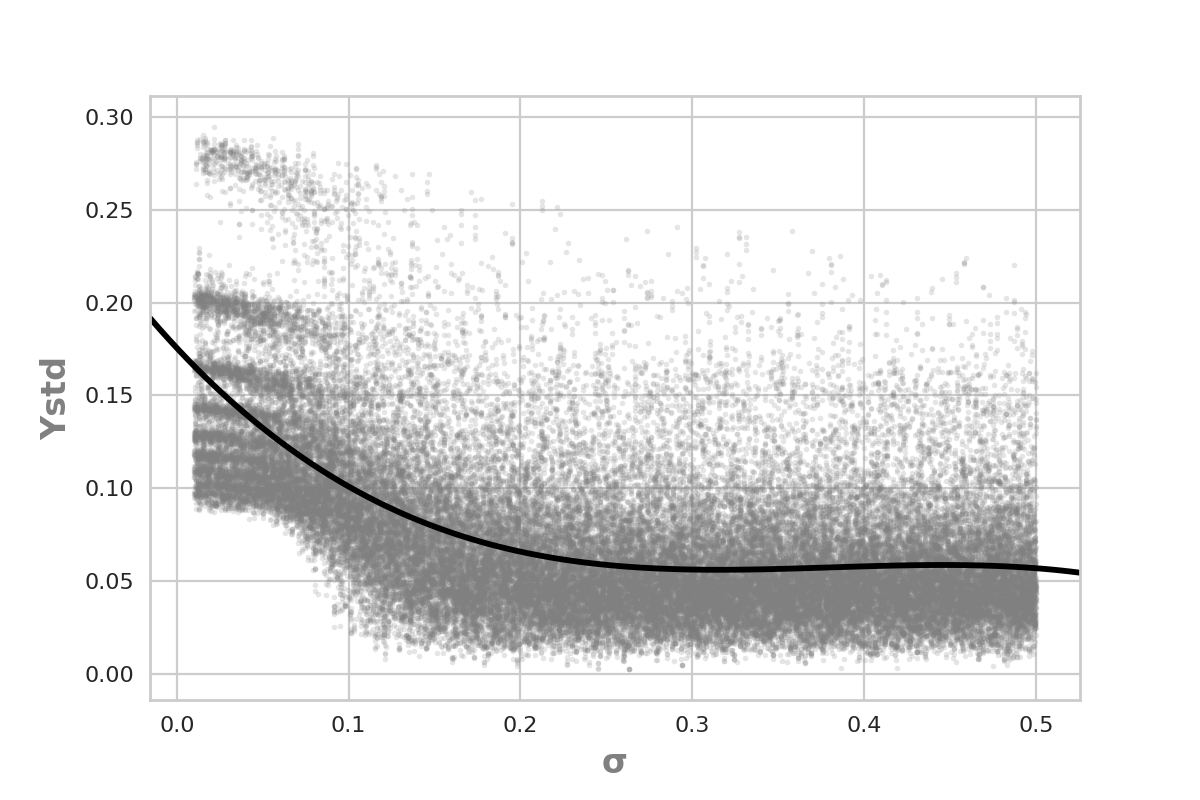
\includegraphics[width=\textwidth]{ims/nlregressions/nlregressionmutatingosigma.png}
          \end{subfigure}
                \begin{subfigure}[b]{0.49\textwidth}
            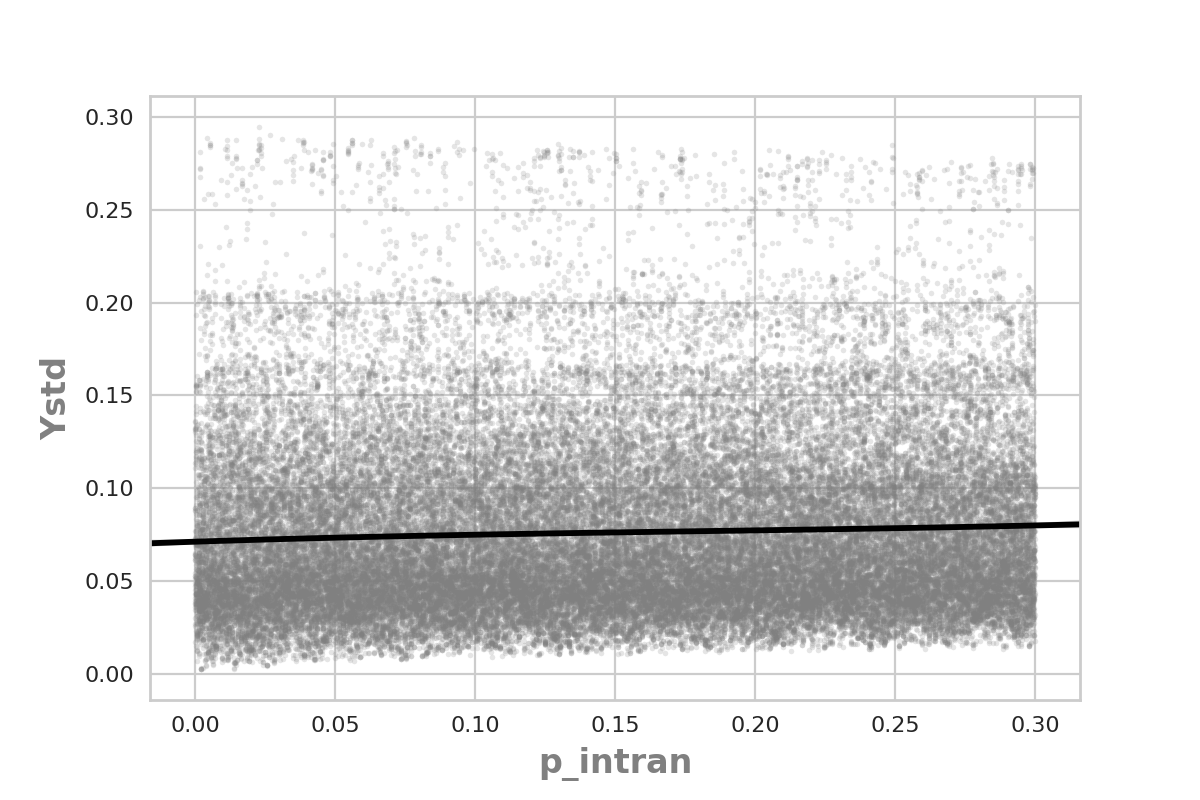
\includegraphics[width=\textwidth]{ims/nlregressions/nlregressionmutatingop_intran.png}
    \end{subfigure}
    \caption{Gráfico de dispersão e regressões polinomiais para 70.000 parametrizações.}
    \label{fig:scatter2}
    \fonte{ O autor.}
  \end{figure}


%%% Local Variables:
%%% mode: latex
%%% TeX-master: "master"
%%% End:
